  \documentclass[journal,12pt,twocolumn]{article}
\usepackage{blindtext}
\usepackage{graphicx}
\graphicspath{{./figs/}}
\usepackage{amsmath,amssymb,amsfonts,amsthm}
\usepackage{watermark}
\newcommand{\myvec}[1]{\ensuremath{\begin{pmatrix}#1\end{pmatrix}}}

\let\vec\mathbf
\thiswatermark{\centering \put(-20,-55){
\includegraphics[scale=0.5]{iith.png}} }
\begin{document}
\title
{Matrix-Lines}
\author{mohammad imran}

\maketitle
\tableofcontents
\bigskip
\section{Problem Statement}
straight line L through point (3,-2) is inclined at an angle of 60 degres to the line  $\surd3x+y=1$.if also intersects the x axis, then equation of L is ?\\
\section{Construction}
\begin{figure}[h]
    \centering
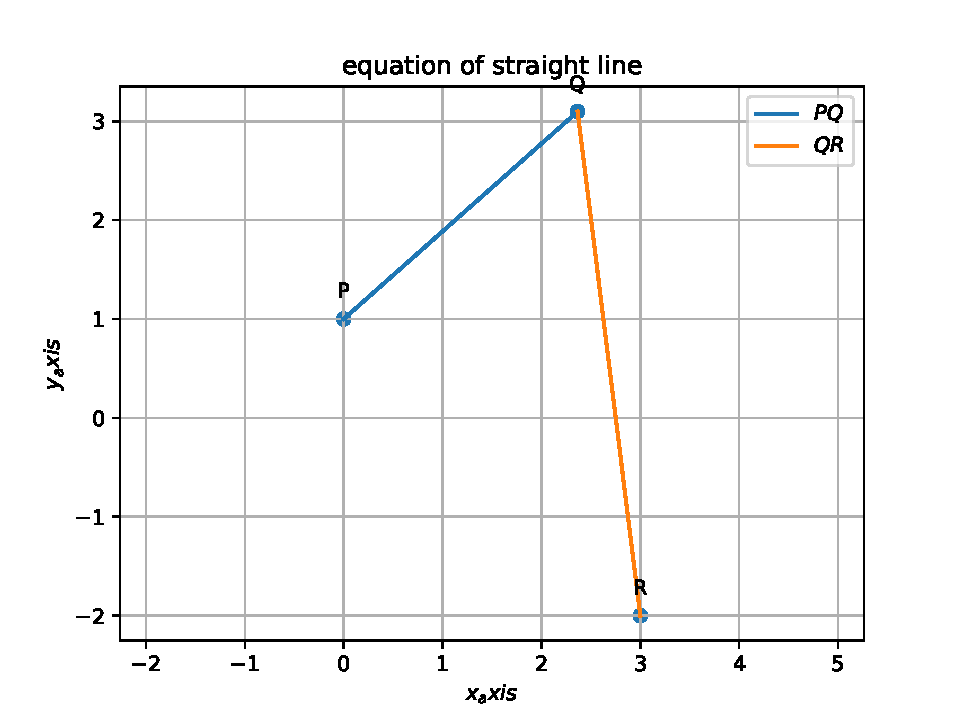
\includegraphics[width=\columnwidth]{figure.pdf}
    \caption{Equation of the Straight Line}
    \label{fig:my_label}
\end{figure}
\vspace{2cm}
\begin{table}[h]
    \centering
    \begin{tabular}{|c|c|c|}
       \hline
       \textbf{Symbol}&\textbf{Value}&\textbf{Description}  \\
       \hline
	    $\vec{P}$ & $\myvec{
		    0\\
		    1}$
	    & Point on Y-axis\\
        \hline
	    $\vec{Q}$ & $\myvec{2.4\\3.1}$
 & Point of Intersection\\
        \hline
	    $\vec{R}$ & $\myvec{
  3\\
  -2}$
 & Given Point \\
        \hline
        $\theta $ & 60  & Given Condition\\
        \hline
         $\vec{a}$ & -
	    & Point on X-axis \\
	    \hline
	    $\vec{e_1}$ & $\myvec{1 \\ 0}$
	    & basic vector\\
	    \hline
    \end{tabular}
    \caption{Parameters}
    \label{tab:my_label}
\end{table}


\section{Solution}
Given that resultant line passes through point(3,-2) and intercepts on x axes and inclined at an angle of 60 degres (let x intercept is (x,0)) \\
\\
%so, b = 9 - a  \\
\\
Let ${\vec{P}}$=$\myvec{
  0\\
  1}$
 , ${\vec{Q}}$=$\myvec{
  2.4\\
  3.1}$
  , ${\vec{R}}$=$\myvec{
  3\\
  -2}$
  ,${\vec{e_1}}=\myvec{1 \\ 0}$
\\
\\
Equation of line is ${\vec{n^{\top}}\vec{X}} = \vec{c}$.\\
\\
the above equation can be written as \center{${\vec{X^{\top}}}\vec{n}=\vec{c}$}\\
 \vspace{0.5cm
 }
 by given point $\vec{R}$ we can write equation of the line as
\begin{equation}
	\myvec{
  3 &
  -2}\vec{n_1}
  = 1 \label{eq-1}
\end{equation}
\\given statement that the line intersects on x axis let point of interscetion be $\vec{a}$
\\
\begin{equation}
\vec{ae_1^{\top}n_1}=1
\end{equation}
\\
by sloving
\begin{equation}
\myvec{1 & 0}n_1=\frac{1}{a}
\end{equation}
%Given Equation of line is $\surd3x+y=1$ \\
%let denote the as Equation of line is ${\vec{n_2^{\top}}\vec{X}} = 1$.\\

%\begin{equation}
%	\vec{n_2^{\top}}
 %    \myvec{
 %\surd3\\ 
 %1} = 1 \label{eq-2}
 %\\
%\begin{equation}
%	\vec{n_2}=
 %    \myvec{
 %\surd3 &&
 %1}  \label{eq-2}
 %\end{equation}
%\\
From eq1 and eq3,\\
\begin{equation}
	\myvec{
  3 & -2\\
  1 & 0
}\vec{n_1}
  = \myvec{1\\
  \frac{1}{a}}   \label{eq-4}
\end{equation}
\\
\begin{equation}
	 \vec{n_1} = 
	 \myvec{
  3 & -2\\
  1 & 0
 }
  ^{-1}
  .
	 \myvec{
  1\\
  \frac{1}{a}}
  \label{eq-7}
\end{equation}
by solving the matric we get \\
\begin{equation}
	\vec{n_1}=
	\myvec{
  \frac{1}{a}  \\  
  \frac{3-a}{2a}}
  \label{eq-8}  
\end{equation}
from given equation of line
\begin{equation}
\myvec{\sqrt{3} & 1}\vec{X}=1
\end{equation}
\begin{equation}
\vec{n_2}=\myvec{\sqrt{3} \\ 1}
\end{equation}
 Angle between two vectors is
 
 \vspace{0.2cm}
 \begin{equation}
 cos\theta=\frac{\vec{n_1^{\top}} \vec{n_2}}{||\vec{n_1}||||\vec{n_2}||}
\end{equation} 

\begin{equation}
 cos60=\frac{\myvec{
  \frac{1}{a}&
  \frac{3-a}{2a}}   \myvec{
 \sqrt{3}\\
 1}}{\sqrt{\myvec{
  \frac{1}{a}}^{2}+\myvec{
  \frac{3-a}{2a}}^{2}}2}
\end{equation}
From angle between two vectors by solving we get the unknown a
\begin{center}
 $\textbf{a}=\frac{2}{\sqrt{3}}+3$
 \end{center} 
 
 \textbf{Put} $a=\frac{2}{\sqrt{3}}+3$   in  eq 6 \\
 
 \begin{equation}
	 \vec{n_1} = 
	 \myvec{\frac{\surd3}{2+3\surd3} \\ \frac{-1}{2+3\sqrt{3}}} 	 
  \label{eq-8}
\end{equation}
by solving we get
 \begin{equation}
	 \vec{n_1} = 
	 \frac{1}{2+3\vec{\sqrt{3}}}\myvec{\sqrt{3} \\ -1}	 
  \label{eq-8}
\end{equation}
The Resultant Equation of line is ${\vec{n_1^{\top}}\vec{X}} = 1$ \\
\vspace{0.5cm}
\textbf{
Desired equation of the line is, }\\
\begin{equation}
\frac{1}{2+\sqrt{3}}\myvec{\sqrt{3} & -1}\vec{X}=1
\end{equation}
      Or,
\begin{equation}
  \myvec{
 \surd3 &&
 -1} \vec{X}=2+3\sqrt{3}
\end{equation}

%   \textbf{ $\surd3x - y = 2+3\surd3$}
%\end{center}
\section{Software}
Download the following code using,
\begin{table}[h]
    \centering
    \begin{tabular}{|c|}
    \hline \\
         https://github.com/imran111888/fwc2/blob//matrix/line/20assignment/codes/1 \\
         \\
\hline
    \end{tabular}
\end{table}
\\
and execute the code by using command
\begin{center}
\textbf{Python3  line.py}\\
\end{center}

\section{Conclusion}
We found the equation of a line passing trough a point
(3,-2) and intersects the x axis.

\end{document}
